\documentclass{article}
\usepackage[utf8]{inputenc}

\title{Space Systems Lab Firmware and Safety Verification}
\author{Hersch Nathan}
\date{November 2024}

\usepackage{url}
\usepackage{float}
\usepackage{natbib}
\usepackage{graphicx}
\usepackage{listings}
\usepackage{fullpage}
\usepackage{hyperref}
\hypersetup{
    colorlinks=true,
    linkcolor=blue,
    filecolor=magenta,      
    urlcolor=cyan,
}

\begin{document}

\maketitle

\section{General Requirements}
\par This software is to support the KRUPS missions. The current mission is KRUPS Aboard Norwegian GhostSat (KANGS).

\section{Architecture Design}
\par The firmware's framework is designed to be modular and configerable for each mission and each hardware. 

\begin{figure} [H]
    \centering
    \caption{Firmware Architecture}
    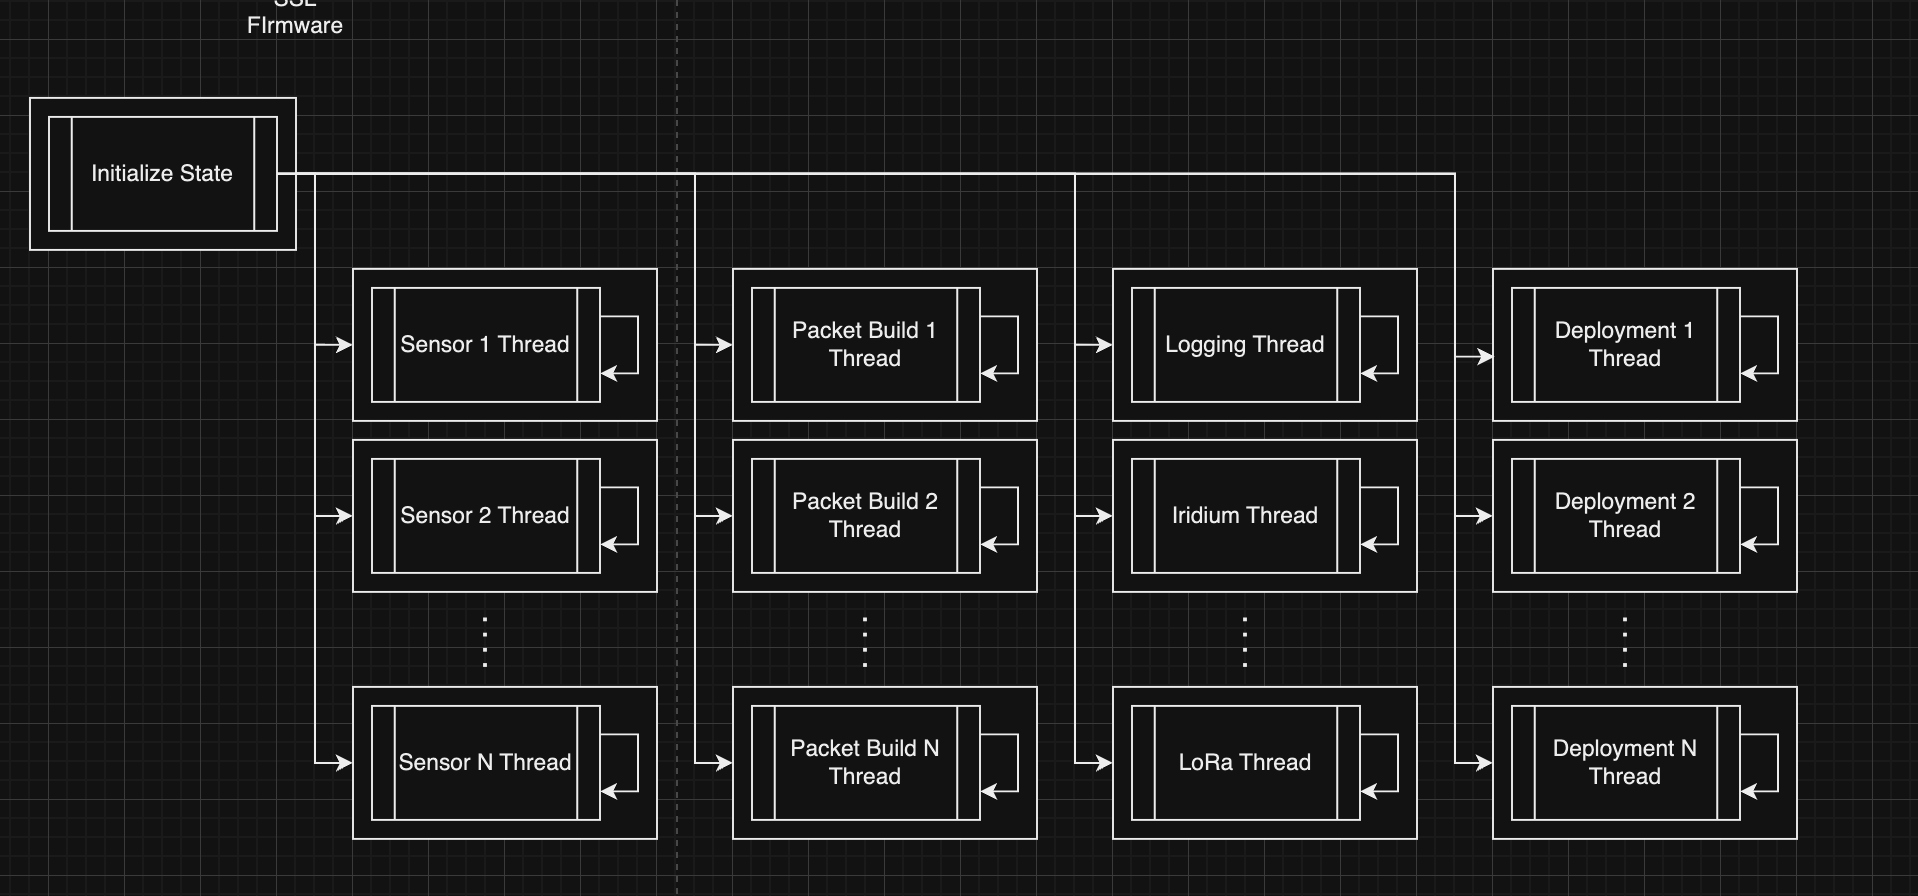
\includegraphics[width=0.8\textwidth]{images/firmware-architecture.png}
    \label{fig:firmware-architecture} 
\end{figure}

\section{Kentucky Flight Computer (KFC) Requirements}

\section{FemptoSats Requirements}
\par The FemptoSats submission is to test the viability of using Wifi/LoRa for intercapsuole communication. 

\subsection{Sensors Requirements}
\par The FemptoSats will have the following sensors: 
\begin{itemize}
    \item BME280 Temperature/pressure/humidity sensor
    \item BNO086 9 - Axis IMU
\end{itemize}

\subsubsection{BME280 Temperature/pressure/humidity sensor}
\par The BME280 will be run with the following configuration settings: 

\subsubsection{BNO086 9 - Axis IMU}
\par The BNO086 will be run with the following configuration settings:

\subsection{Wireless Communcation Requirements}
\par the FemptoSat will use the following Wireless Communcation modules:
\begin{itemize}
    \item Integrated Wifi
    \item LoRa
\end{itemize}
\par The Wifi will fail over to the LoRa when the Wifi gets out of range

\section{Rocketstation Transmitter (RST) Requirements}

\section{Rocketstation Requirements}

\section{Groundstation Requirements}




%%%%%%%%%%%%%%%%%%%%%%%%%%%%%%%%%%%%%%%%%%%%%%%%%%%%%%%%%%%%%%%%%%%%%%%%%%%%%%%%%%%
%%%%%%%%%%%%%%%%%%%%%%%%%%%%%%%%%%%%%%%%%%%%%%%%%%%%%%%%%%%%%%%%%%%%%%%%%%%%%%%%%%%
%%%%%%%%%%%%%%%%%%%%%%%%%%%%%%%%  APPENDIX
%%%%%%%%%%%%%%%%%%%%%%%%%%%%%%%%%%%%%%%%%%%%%%%%%%%%%%%%%%%%%%%%%%%%%%%%%%%%%%%%%%%
%%%%%%%%%%%%%%%%%%%%%%%%%%%%%%%%%%%%%%%%%%%%%%%%%%%%%%%%%%%%%%%%%%%%%%%%%%%%%%%%%%%
%\appendix

%\newpage
%\section{Arduino Pin Mapping}
%\label{app:pinmap}
%\lstinputlisting[language={}]{arduino-pinmap.txt}

%\bibliographystyle{plain}
%\bibliography{references}
\end{document}
